\chapter{有界线性算子}
\vspace{-2em}

本章将更详细地考察Banach空间中的线性算子.如第2章一样， $\mathcal{B}\left( {X,Y}\right)$ 表示所有有界线性算子 $\Lambda  : X \mapsto  Y$ 构成的空间，其范数为
\[
\| \Lambda \|  \doteq  \mathop{\sup }\limits_{{\| x\|  \leq  1}}\| {\Lambda x}\| .
\]

我们首先给出一些基于Baire纲定理的结果.

\section{一致有界性原理}

\begin{theorem}[Banach-Steinhaus一致有界性原理]\label{thm:banach-steinhaus}
设 $X,Y$ 为Banach空间， $\mathcal{F} \subset  \mathcal{B}\left( {X,Y}\right)$ 为一族有界线性算子.则要么 $\mathcal{F}$ 是一致有界的，即
\[
\mathop{\sup }\limits_{{\Lambda  \in  \mathcal{F}}}\| \Lambda \|  < \infty ,
\]
要么存在一个稠密集 $S \subset  X$ ，使得
\begin{equation}\tag{4.1}\label{eq:unif-bddness-blowup}
\mathop{\sup }\limits_{{\Lambda  \in  \mathcal{F}}}\| {\Lambda x}\|  = \infty ,\;\forall\,x \in  S.
\end{equation}
\end{theorem}

\begin{proof}
对每个整数 $n$ ，考虑开集
\begin{equation}\tag{4.2}\label{eq:Sn-def}
{S}_{n} \doteq  \{ x \in  X;\exists\,\Lambda\in\mathcal{F},\| {\Lambda x}\|  > n\} .
\end{equation}

若这些集合中有一个(比如 ${S}_{k}$ )在 $X$ 中不稠密，则存在 ${x}_{0} \in  X$ 和半径 $r > 0$ ，使得闭球 $\bar{B}\left( {{x}_{0},r}\right)$ 与 ${S}_{k}$ 不相交.换言之，
\[
\| {\Lambda x}\|  \leq  k\forall\,\Lambda  \in  \mathcal{F},\;x \in  \bar{B}\left( {{x}_{0},r}\right) .
\]

若此时 $\| x\|  \leq  r$ ，则
\[
\| {\Lambda x}\|  = \norm{\Lambda \left( {{x}_{0} + x}\right)  - \Lambda {x}_{0}} \leq  \norm{\Lambda \left( {{x}_{0} + x}\right) } + \norm{\Lambda {x}_{0}} \leq  {2k}
\]
对所有 $\Lambda  \in  \mathcal{F}$ 成立.因此
\[
\| \Lambda \|  \doteq  \mathop{\sup }\limits_{{\| x\|  \leq  1}}\| {\Lambda x}\|  = \frac{1}{r}\mathop{\sup }\limits_{{\| x\|  \leq  r}}\| {\Lambda x}\|  \leq  \frac{2k}{r}
\]
对每个 $\Lambda  \in  \mathcal{F}$ 成立.此时，算子族 $\mathcal{F}$ 一致有界.

另一种可能是:式\eqref{eq:Sn-def}中的开集 ${S}_{n}$ 全都在 $X$ 中稠密.由Baire纲定理，交集 $S \doteq  \mathop{\bigcap }\limits_{{n \geq  1}}{S}_{n}$ 在 $X$ 中稠密.由构造可知，对每个 $x \in  S$ 和 $n \geq  1$ ，均存在算子 $\Lambda  \in  \mathcal{F}$ ，使得 $\| {\Lambda x}\|  > n$ 成立.故\eqref{eq:unif-bddness-blowup}成立.
\end{proof}

\begin{remark}\label{rem:uniform-boundedness-pointwise}
由定理\ref{thm:banach-steinhaus}可知，若算子族 $\Lambda  \in  \mathcal{B}\left( {X,Y}\right)$ 在单位球上逐点有界，则其一致有界.换言之，条件
\[
\mathop{\sup }\limits_{{\Lambda  \in  \mathcal{F}}}\| {\Lambda x}\| \, < \,\infty \;\text{ for each }x \in  X\text{ with }\| x\|  \leq  1
\]
蕴含
\[
\mathop{\sup }\limits_{{\Lambda  \in  \mathcal{F}}}\mathop{\sup }\limits_{{\| x\|  \leq  1}}\| {\Lambda x}\|  < \infty .
\]
这正是“一致有界性原理”这一名称的由来.
\end{remark}

\begin{corollary}[逐点极限的连续性]\label{cor:pointwise-limit-continuous}
设 $X,Y$ 为Banach空间， ${\left( {\Lambda }_{n}\right) }_{n \geq  1}$ 是 $\mathcal{B}\left( {X;Y}\right)$ 中一列有界线性算子.假设对每个 $x \in  X$ ，逐点极限
\begin{equation}\tag{4.3}\label{eq:pointwise-limit-def}
{\Lambda x} \doteq  \mathop{\lim }\limits_{{n \rightarrow  \infty }}{\Lambda }_{n}x
\end{equation}
均存在.则由\eqref{eq:pointwise-limit-def}定义的映射 $\Lambda$ 是一个有界线性算子.
\end{corollary}

\begin{proof}
对每个 $x \in  X$ ，序列 ${\left( {\Lambda }_{n}x\right) }_{n \geq  1}$ 有界.故由定理\ref{thm:banach-steinhaus}，序列 ${\Lambda }_{n}$ 一致有界.这表明
\[
\| \Lambda \|  \doteq  \mathop{\sup }\limits_{{\| x\|  \leq  1}}\| {\Lambda x}\|  = \mathop{\sup }\limits_{{\| x\|  \leq  1}}\left( {\mathop{\lim }\limits_{{n \rightarrow  \infty }}\norm{{\Lambda }_{n}x}}\right)  \leq  \mathop{\sup }\limits_{{n \geq  1}}\norm{{\Lambda }_{n}} < \infty ,
\]
从而说明线性算子 $\Lambda$ 有界.
\end{proof}

\section{开映射定理}

\begin{definition}[开映射]
    设$X,Y$ 是度量空间，若映射 $f : X \mapsto  Y$满足：对每个开子集 $U \subseteq  X$ ，其像 $f\left( U\right)$ 是 $Y$ 的开子集，则称$f$是\colorbf{开映射}.
\end{definition}
该性质成立当且仅当:对每个 $x \in  X$ 和 $r > 0$ ，以 $x$ 为中心、半径为 $r > 0$ 的开球的像 $f\left( {B\left( {x,r}\right) }\right)$ 包含一个以 $f\left( x\right)$ 为中心的球.

\begin{theorem}[开映射定理]\label{thm:open-mapping}
设 $X,Y$ 是Banach空间， $\Lambda  : X \mapsto \; Y$ 是一个有界满射线性算子，则 $\Lambda$ 是开映射.
\end{theorem}

\begin{proof}
1．由线性性，开球 $B\left( {x,r}\right)$ 的像可表示为
\[
\Lambda \left( {B\left( {x,r}\right) }\right)  = \Lambda \left( x\right)  + \Lambda \left( {B\left( {0,r}\right) }\right)  = \Lambda \left( x\right)  + {r\Lambda }\left( {B\left( {0,1}\right) }\right) .
\]

设 ${B}_{r} \doteq  B\left( {0,r}\right)$ 为以原点为中心、半径为 $r$ 的开球，因此为证明该定理，只需证像集 $\Lambda \left( {B}_{1}\right)$ 包含 $Y$ 中一个以原点为中心的开球.

\noindent 2. 由于 $\Lambda$ 是满射，故 $Y = \mathop{\bigcup }\limits_{{n = 1}}^{\infty }\Lambda \left( {B}_{n}\right)$ .回顾 $Y$ 是完备度量空间，由Baire定理可知，至少有一个闭包 $\overline{\Lambda \left( {B}_{n}\right) } \subset  Y$ 具有非空内部.

通过缩放论证， $\overline{\Lambda \left( {B}_{1}\right) } = {n}^{-1}\overline{\Lambda \left( {B}_{n}\right) }$ 也必具有非空内部.即存在 ${y}_{0} \in  Y$ 与 $r > 0$，使得 $B\left( {{y}_{0},r}\right)  \subset  \overline{\Lambda \left( {B}_{1}\right) }$ .

由于开单位球 ${B}_{1}$ 是凸集且对称，其像集 $\Lambda \left( {B}_{1}\right)$ 及闭包 $\overline{\Lambda \left( {B}_{1}\right) }$ 亦然.特别地，由对称性得 $B\left( {-{y}_{0},r}\right)  \subseteq  \overline{\Lambda \left( {B}_{1}\right) }$ ，而凸性则意味着球 $B\left( {0,r}\right)  \subset  Y$ 满足
\[
B\left( {0,r}\right)  = \frac{1}{2}B\left( {{y}_{0},r}\right)  + \frac{1}{2}B\left( {-{y}_{0},r}\right)  \subseteq  \overline{\Lambda \left( {B}_{1}\right) }.
\]

再次利用 $\Lambda$ 的线性性，经缩放可得
\begin{equation}\tag{4.4}\label{eq:open-mapping-scaled-balls}
B\left( {0,{2}^{-n}r}\right)  \subseteq  \overline{\Lambda \left( {B}_{{2}^{-n}}\right) }\forall\,n \geq  1.
\end{equation}

\noindent 3. 我们通过证明 $B\left( {0,r/2}\right)  \subseteq  \Lambda \left( {B}_{1}\right)$ 来完成证明.事实上，任取一点 $y \in  B\left( {0,r/2}\right)$ ，我们采用归纳法.

\begin{itemize}
    \item 由稠密性，可找到 ${x}_{1} \in  {B}_{{2}^{-1}}$ 使得 $\norm{y - \Lambda {x}_{1}} < {2}^{-2}r$ .
    \item 反之，我们可以找到 ${x}_{2} \in  {B}_{{2}^{-2}}$ ，使得 $\norm{\left( {y - \Lambda {x}_{1}}\right)  - \Lambda {x}_{2}} < {2}^{-3}r$ .
    \item 继续用归纳法，对每个 $n$ ，均有\[
y - \mathop{\sum }\limits_{{j = 1}}^{{n - 1}}\Lambda {x}_{j} \in  B\left( {0,{2}^{-n}r}\right)  \subseteq  \overline{\Lambda \left( {B}_{{2}^{-n}}\right) }.
\]
\end{itemize}

因此可选取一点 ${x}_{n} \in  {B}_{{2}^{-n}}$ ，使得
\[
\norm{\left( {y - \mathop{\sum }\limits_{{j = 1}}^{{n - 1}}\Lambda {x}_{j}}\right)  - \Lambda {x}_{n}} < {2}^{-n - 1}r.
\]

由于 $X$ 是 Banach 空间且 $\mathop{\sum }\limits_{n}\norm{x}_{n} < \infty$ ，级数 $\mathop{\sum }\limits_{n}{x}_{n}$ 收敛，设其和为 $\mathop{\sum }\limits_{{n = 1}}^{\infty }{x}_{n} = x$.我们注意到
\[
\| x\|  \leq  \mathop{\sum }\limits_{{n = 1}}^{\infty }\norm{x}_{n} < \mathop{\sum }\limits_{{n = 1}}^{\infty }{2}^{-n} = 1,\;{\Lambda x} = \mathop{\lim }\limits_{{n \rightarrow  \infty }}\mathop{\sum }\limits_{{j = 1}}^{n}\Lambda {x}_{j} = y.
\]

故像集 $\Lambda \left( {B}_{1}\right)$ 包含所有满足 $\| y\|  < r/2$ 的点 $y \in  Y$ .
\end{proof}

\begin{corollary}\label{cor:inverse-continuous}
设$X,Y$ 是 Banach 空间，且$\Lambda  : X \mapsto  Y$是连续双射，则逆映射${\Lambda }^{-1} : Y \mapsto  X$ 连续.
\end{corollary}

\begin{proof}
由于 $\Lambda$ 是双射， $\Lambda$ 是开映射当且仅当逆映射 ${\Lambda }^{-1}$ 连续.
\end{proof}

\section{闭图像定理}

设 $X,Y$ 是 Banach 空间.乘积空间 $X \times  Y$ 是所有有序对 $\left( {x,y}\right)$ 的集合，其中 $x \in  X$ 且 $y \in  Y$ .该空间按如下范数构成 Banach 空间:
\begin{equation}\tag{4.5}\label{eq:product-norm}
\| \left( {x,y}\right) \|  \doteq  \| x\|  + \| y\| .
\end{equation}

接下来，设 $\Lambda$ 是一个(可能无界)线性算子，定义域为 $\operatorname{Dom}\left( \Lambda \right)  \subseteq \; X$ ，取值于 $Y$.若其图像
\[
\operatorname{Graph}\left( \Lambda \right)  \doteq  \left\{  {\left( {x,y}\right) ;x \in  \operatorname{Dom}\left( \Lambda \right)  \subseteq  X,y = {\Lambda x}}\right\}   \subset  X \times  Y
\]
是乘积空间 $X \times  Y$ 的闭子集，则称 $\Lambda$ 是闭的.换言之，线性算子 $\Lambda$ 是闭的，当且仅当下列条件成立:
\begin{definition}[闭算子]
    设$X,Y$ 是 Banach 空间， $\Lambda : X \mapsto  Y$ 是一个线性算子，称$\Lambda$是\colorbf{闭线性算子}，若其满足以下任一等价条件：
    \begin{enumerate}[(i)]
        \item 其图像 $\operatorname{Graph}\left( \Lambda \right)$ 是 $X \times  Y$ 的闭子集.
        \item 对任意序列${x}_{n} \in  \operatorname{Dom}\left( \Lambda \right)$ 和 ${y}_{n} = \Lambda {x}_{n} \in  Y$ ，若 ${x}_{n} \rightarrow  x$ 且 ${y}_{n} \rightarrow  y$ ，则必有 $x \in  \operatorname{Dom}\left( \Lambda \right)$ 且 ${\Lambda x} = y$ .
    \end{enumerate}
\end{definition}


注意，每个连续线性算子 $\Lambda  : X \mapsto  Y$ 均为闭算子.下一个结果表明:若定义域 $\operatorname{Dom}\left( \Lambda \right)$ 恰为全空间 $X$ ，则其逆命题亦成立.

\begin{theorem}[闭图像定理]\label{thm:closed-graph}
设 $X,Y$ 是 Banach 空间， $\Lambda : X \mapsto  Y$ 是定义在整个空间 $X$ 上的闭线性算子，则 $\Lambda$ 连续.
\end{theorem}

\begin{proof}
记 $\Gamma  \doteq  \operatorname{Graph}\left( \Lambda \right)$ .由假设， $\Gamma$ 是 Banach 空间 $X \times  Y$ 的闭子空间，故其本身也是 Banach 空间.

考虑投影映射 ${\pi }_{1} : \Gamma  \mapsto  X$ 和 ${\pi }_{2} : \Gamma  \mapsto  Y$ ，定义为
\[
{\pi }_{1}\left( {x,{\Lambda x}}\right)  = x,\;{\pi }_{2}\left( {x,{\Lambda x}}\right)  = {\Lambda x}.
\]

映射 ${\pi }_{1}$ 是 $\Gamma$ 与 $X$ 之间的双射，因此由推论\ref{cor:inverse-continuous}，其逆映射 ${\pi }_{1}^{-1}$ 连续.故 $\Lambda  = {\pi }_{2} \circ  {\pi }_{1}^{-1}$ 是两个连续映射的复合，从而连续.
\end{proof}

\begin{figure}[htbp]
\centering
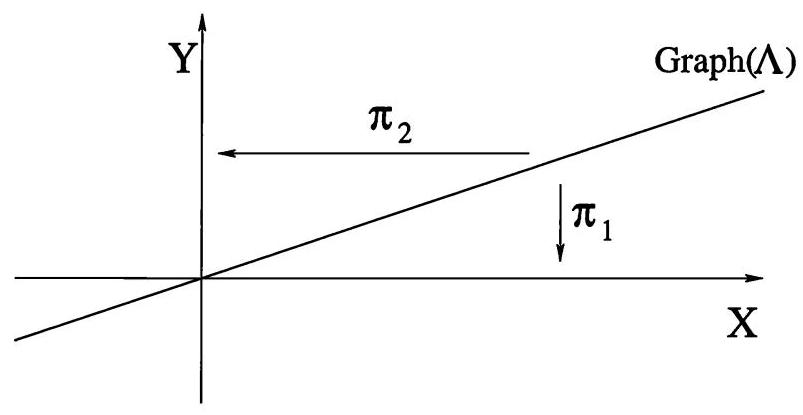
\includegraphics[width=0.65\textwidth]{images/bo_d6ik6nn7aajc739ct1l0_77_338_701_803_415_0.jpg}
\caption{闭图像定理的证明.}
\label{fig:closed-graph-proof}
\end{figure}

\begin{instance}\label{ins:derivative-operator-not-bounded-but-closed}
考虑所有有界连续函数 $f : \mathbb{R} \mapsto  \mathbb{R}$ 构成的空间 $X = {\mathcal{C}}^{0}\left( \mathbb{R}\right)$ ，其范数为 $\| f{\| }_{{\mathcal{C}}^{0}} \doteq  \mathop{\sup }\limits_{x}\left| {f\left( x\right) }\right|$ .令 $\Lambda$ 为由 ${\Lambda f} = {f}^{\prime }$ 定义的微分算子.其定义域为如下子空间
\[
\operatorname{Dom}\left( \Lambda \right)  = \left\{  {f \in  {\mathcal{C}}^{0}\left( \mathbb{R}\right) ;{f}^{\prime } \in  {\mathcal{C}}^{0}\left( \mathbb{R}\right) }\right\}   = {\mathcal{C}}^{1}\left( \mathbb{R}\right)
\]
---即所有导数有界的连续可微函数构成的子空间.

注意，线性算子 $\Lambda$ 不是有界的(因而不连续).例如，函数列 ${f}_{n}\left( x\right)  = \sin {nx}$ 一致有界:对所有 $n \geq  1$ ，均有 ${\norm{f}_{n}}_{{\mathcal{C}}^{0}} = 1$ .然而，其导数序列 $\Lambda {f}_{n} = {f}_{n}^{\prime }$ 无界，因为 ${f}_{n}^{\prime }\left( x\right)  = n\cos {nx}$ ，故 ${\norm{f}_{n}^{\prime }}_{{\mathcal{C}}^{0}} = n$ .

另一方面，线性算子 $\Lambda  : f \mapsto  {f}^{\prime }$ 具有闭图像.为证此，考虑序列 ${f}_{n} \in  \operatorname{Dom}\left( \Lambda \right)$ ，使得对某些函数 $f,g \in  {\mathcal{C}}^{0}$ ，有
\begin{equation}\tag{4.6}\label{eq:derivative-graph-closed}
{\norm{f}_{n} - f}_{{\mathcal{C}}^{0}} \rightarrow  0,\;{\norm{f}_{n}^{\prime } - g}_{{\mathcal{C}}^{0}} \rightarrow  0.
\end{equation}

若\eqref{eq:derivative-graph-closed}成立，则 $f$ 连续可微，且 ${f}^{\prime } = g$ .因此点 $\left( {f,g}\right)  \in  X \times  X$ 属于 $\Lambda$ 的图像.

注意，该例并不与定理\ref{thm:closed-graph}矛盾，因为 $\Lambda$ 并未在整个空间 $X$ 上定义.
\end{instance}

\section{伴随算子}

设 $X$ 是域 $\mathbb{K}$ 上的Banach空间.依定义，其对偶空间是所有有界(因而连续)线性泛函 ${x}^{ * } : X \mapsto  \mathbb{K}$ 构成的空间 ${X}^{ * }$ ，其范数为
\[
\norm{x}^{ * } \doteq  \mathop{\sup }\limits_{{\| x\|  \leq  1}}\left| {{x}^{ * }\left( x\right) }\right| .
\]

反过来，每个元素 $x \in  X$ 均在 ${X}^{ * }$ 上诱导一个有界线性泛函，即 ${x}^{ * } \mapsto  {x}^{ * }\left( x\right)  \in  \mathbb{K}$.利用这一等同关系，我们可写作 $X \subseteq \; {\left( {X}^{ * }\right) }^{ * }$ .由于空间 $X$ 与 ${X}^{ * }$ 常扮演对称角色，采用记号
\[
\left\langle  {{x}^{ * },x}\right\rangle   \doteq  {x}^{ * }\left( x\right) .
\]
设 $X,Y$ 为域 $\mathbb{K}$ 上的Banach空间， ${X}^{ * },{Y}^{ * }$ 为其对偶空间.设 $\Lambda  : X \mapsto  Y$ 为有界线性算子.则对任意有界线性泛函 ${y}^{ * } : Y \mapsto  \mathbb{K}$ ，由 ${x}^{ * } : X \mapsto  \mathbb{K}$ 定义的复合映射 ${x}^{ * }\left( x\right)  = {y}^{ * }\left( {\Lambda x}\right)$ 是 $X$ 上的有界线性泛函.映射 $\Lambda^*:{y}^{ * } \mapsto  {\Lambda }^{ * }{y}^{ * } \doteq  {y}^{ * } \circ  \Lambda$ 是从 ${Y}^{ * }$ 到 ${X}^{ * }$ 的有界线性算子，称为 $\Lambda$ 的伴随算子.\par
\begin{definition}[伴随算子]
    设 $X,Y$ 为域 $\mathbb{K}$ 上的Banach空间， ${X}^{ * },{Y}^{ * }$ 为其对偶空间.设 $\Lambda  : X \mapsto  Y$ 为有界线性算子.则对任意有界线性泛函 ${y}^{ * } : Y \mapsto  \mathbb{K}$ ，由 ${x}^{ * } : X \mapsto  \mathbb{K}$ 定义的复合映射 ${x}^{ * }\left( x\right)  = {y}^{ * }\left( {\Lambda x}\right)$唯一确定$Y^*\to X^*$上的有界线性算子$\Lambda^*:{y}^{ * } \mapsto  {\Lambda }^{ * }{y}^{ * } \doteq  {y}^{ * } \circ  \Lambda$，称为 $\Lambda$ 的\colorbf{伴随算子}.
\end{definition}
根据定义(见图\ref{fig:adjoint-maps})，
\[
\left\langle  {{\Lambda }^{ * }{y}^{ * },x}\right\rangle   = \left\langle  {{y}^{ * },{\Lambda x}}\right\rangle,\;\forall\,x \in  X.
\]

以下，对给定子集 $V \subseteq  X$ ，我们将其正交集定义为
\[
{V}^{ \bot  } \doteq  \left\{  {{x}^{ * } \in  {X}^{ * };\left\langle  {{x}^{ * },x}\right\rangle   = 0,\forall\,x \in  V}\right\}  .
\]

类似地，若 $W \subseteq  {X}^{ * }$ ，我们定义
\[
{W}^{ \bot  } \doteq  \left\{  {x \in  X;\left\langle  {{x}^{ * },x}\right\rangle   = 0,\forall\,{x}^{ * } \in  W}\right\}  .
\]

\begin{figure}[htbp]
\centering
\begin{tikzcd}[labels={font=\normalsize}]
X \arrow[rr, "\Lambda"] &  & Y                            &  & X \arrow[rr, "\Lambda"] \arrow[rrdd, "\Lambda^*y^*"'] &  & Y \arrow[dd, "y^*"] \\
                        &  &                              &  &                                                       &  &                     \\
X^*                     &  & Y^* \arrow[ll, "\Lambda^*"'] &  &                                                       &  & \mathbb{K}         
\end{tikzcd}
\captionof{figure}{伴随算子定义中涉及的映射.}
\label{fig:adjoint-maps}
\end{figure}

\begin{theorem}[伴随算子的性质]\label{thm:adjoint-properties}
设 $\Lambda  : X \mapsto  Y$ 为有界线性算子， ${\Lambda }^{ * } : {Y}^{ * } \mapsto  {X}^{ * }$ 为其伴随算子.则:

(i) $\norm{{\Lambda }^{ * }} = \| \Lambda \|$ .

(ii) $\operatorname{Ker}\left( \Lambda \right)  = {\left(  \operatorname{Range}\left( {\Lambda }^{ * }\right) \right)  }^{ \bot  }$ 且 $\operatorname{Ker}\left( {\Lambda }^{ * }\right)  = {\left(  \operatorname{Range}\left( \Lambda \right) \right)  }^{ \bot  }$ .
\end{theorem}

\begin{proof}
(i) 由下式推出
{\setjot[-2]\begin{align*}
    \| \Lambda \| &= \sup \left\{  {\| {\Lambda x}\| ;\| x\|  \leq  1}\right\}\\
    &= \sup \left\{  {\left| \left\langle  {{y}^{ * },{\Lambda x}}\right\rangle  \right| ;\| x\|  \leq  1,\norm{y}^{ * } \leq  1}\right\}\\
    &= \sup \left\{  {\left| \left\langle  {{\Lambda }^{ * }{y}^{ * },x}\right\rangle  \right| ;\| x\|  \leq  1,\norm{y}^{ * } \leq  1}\right\}\\
    &= \sup \left\{  {\norm{{\Lambda }^{ * }{y}^{ * }};\norm{y}^{ * } \leq  1}\right\}   = \norm{{\Lambda }^{ * }}.
\end{align*}}
(ii) 我们注意到下列命题彼此等价:
{\setjot[-4]\begin{align*}
    x &\in  \operatorname{Ker}\left( \Lambda \right)\\
    {\Lambda x} &= 0 \\
    \left\langle  {{y}^{ * },{\Lambda x}}\right\rangle   &= 0\ \forall\,{y}^{ * } \in  {Y}^{ * } \\
    \left\langle  {{\Lambda }^{ * }{y}^{ * },x}\right\rangle   &= 0\ \forall\,{y}^{ * } \in  {Y}^{ * }   \\
    x &\in  {\left(  \operatorname{Range}\left( {\Lambda }^{ * }\right) \right)  }^{ \bot  }.
\end{align*}}

类似地，下列命题也彼此等价:
{\setjot[-4]\begin{align*}
    {y}^{ * } &\in  \operatorname{Ker}\left( {\Lambda }^{ * }\right)\\
    {\Lambda }^{ * }{y}^{ * } &= 0\\
    \left\langle  {{\Lambda }^{ * }{y}^{ * },x}\right\rangle   &= 0\ \forall\,x \in  X\\
    \left\langle  {{y}^{ * },{\Lambda x}}\right\rangle   &= 0\ \forall\,x \in  X\\
    {y}^{ * } &\in  {\left(  \operatorname{Range}\left( \Lambda \right) \right)  }^{ \bot  }.
\end{align*}}

\end{proof}

本节最后，我们给出一致有界性原理的一个有用应用.

\begin{corollary}[弱收敛序列必有界]\label{cor:weakly-convergent-bounded}
设 $X$ 为Banach空间，则任何弱收敛于某个 $x \in  X$ 的序列 ${x}_{n} \in  X$ 必为有界序列.
\end{corollary}

\begin{proof}
设 ${X}^{ * }$ 为 $X$ 的对偶空间.每个 ${x}_{n}$ 确定 ${X}^{ * }$ 上的一个线性泛函 ${\psi }_{n}$ ，定义为
\[
{\psi }_{n}\left( {x}^{ * }\right)  \doteq  \left\langle  {{x}^{ * },{x}_{n}}\right\rangle  .
\]
此处 $\langle  \cdot  , \cdot  \rangle$ 表示 $X$ 与 ${X}^{ * }$ 之间的对偶关系.由假设，当 $n \rightarrow  \infty$ 时，逐点收敛
\[
{\psi }_{n}\left( {x}^{ * }\right)  =  \left\langle  {{x}^{ * },{x}_{n}}\right\rangle   \rightarrow  \left\langle  {{x}^{ * },x}\right\rangle
\]
对每个 ${x}^{ * } \in  {X}^{ * }$ 成立.这意味着
\[
\mathop{\sup }\limits_{n}\left| {{\psi }_{n}\left( {x}^{ * }\right) }\right|  < \infty \text{ for every }{x}^{ * } \in  {X}^{ * }.
\]

由定理\ref{thm:banach-steinhaus}可知，线性泛函族 $\left\{  {{\psi }_{n};n \geq  1}\right\}$ 一致有界.又因
\[
\norm{{\psi }_{n}} = \mathop{\sup }\limits_{{\norm{x}^{ * } \leq  1}}\left| {{\psi }_{n}\left( {x}^{ * }\right) }\right|  = \norm{{x}_{n}},
\]
故序列 ${x}_{n}$ 有界.
\end{proof}

\section{紧算子}

\begin{definition}[紧算子]
    设 $X,Y$ 为Banach空间.称有界线性算子 $\Lambda  : X \mapsto  Y$ 为\colorbf{紧算子}，若其满足任一等价条件：
    \begin{enumerate}[(i)]
        \item 对 $X$ 中任意有界点列 ${\left( {x}_{n}\right) }_{n \geq  1}$ ，均存在子列 ${\left( {x}_{{n}_{j}}\right) }_{j \geq  1}$ ，使得 $\Lambda {x}_{{n}_{j}}$ 收敛.
        \item 对 $X$ 中任意有界集 $U$ ，其像 $\Lambda \left( U\right)$ 的闭包 $\overline{\Lambda \left( U\right) }$ 是 $Y$ 中的紧集.
    \end{enumerate}
\end{definition}


\begin{theorem}[紧算子的例子]\label{thm:compact-examples}
(i) 设 $X,Y$ 为Banach空间， $\Lambda  : X \mapsto  Y$ 为有界线性算子.若 $\Lambda$ 的值域是有限维的，则 $\Lambda$ 是紧算子.

(ii) 设 ${\Lambda }_{n} : X \mapsto  Y$ 为紧算子，对每个 $n \geq  1$ 成立.假设 $\mathop{\lim }\limits_{{n \rightarrow  \infty }}\norm{{\Lambda }_{n} - \Lambda } = 0$ .则算子 $\Lambda$ 也是紧的.
\end{theorem}

\begin{proof}
1. 有界线性算子 $\Lambda  : X \mapsto  Y$ 是紧的当且仅当单位球 ${B}_{1} \subset  X$ 的像 $\Lambda \left( {B}_{1}\right)  \subset  Y$ 的闭包是紧的.若 $\operatorname{Range}\left( \Lambda \right)$ 是有限维的且 $\Lambda$ 有界，则闭包 $\overline{\Lambda \left( {B}_{1}\right) }$ 是有限维空间中的闭有界子集，故为紧集.这就证明了 (i).

\noindent 2. 为证 (ii)，我们注意到:由于 $Y$ 完备，闭包 $\overline{\Lambda \left( {B}_{1}\right) }$ 是紧的当且仅当 $\Lambda \left( {B}_{1}\right)$ 是列紧的.这意味着:对任意 $\varepsilon  > 0$ ，集合 $\Lambda \left( {B}_{1}\right)$ 可被有限个半径为 $\varepsilon$ 的球覆盖.

在假设 (ii) 下，给定 $\varepsilon  > 0$ .选取 $k$ 使得 $\norm{\Lambda  - {\Lambda }_{k}} < \varepsilon /2$ .由于 ${\Lambda }_{k}$ 是紧的，可选出有限个元素 ${y}_{1},\ldots ,{y}_{N} \in  Y$ ，使得
\begin{equation}\tag{4.7}\label{eq:compact-covering}
{\Lambda }_{k}\left( {B}_{1}\right)  \subseteq  \mathop{\bigcup }\limits_{{i = 1}}^{N}B\left( {{y}_{i},\frac{\varepsilon }{2}}\right) .
\end{equation}

若 $\| x\|  \leq  1$ ，则 $\norm{{\Lambda x} - {\Lambda }_{k}x} < \varepsilon /2$ .由\eqref{eq:compact-covering}存在一点 ${y}_{i}$ 满足 $\norm{{\Lambda }_{k}x - {y}_{i}} < \varepsilon /2$ .由三角不等式， $\norm{{\Lambda x} - {y}_{i}} < \varepsilon$ .这表明有限个球 $B\left( {{y}_{i},\varepsilon }\right)$ 覆盖了 $\Lambda \left( {B}_{1}\right)$ .
\end{proof}

\begin{theorem}[紧算子的伴随算子]\label{thm:compact-adjoint}
设 $X,Y$ 为Banach空间， $\Lambda  : X \mapsto  Y$ 为有界线性算子.则 $\Lambda$ 是紧算子当且仅当其伴随算子 ${\Lambda }^{ * } : {Y}^{ * } \mapsto  {X}^{ * }$ 是紧算子.
\end{theorem}

\begin{proof}
1. 假设 $\Lambda$ 是紧算子.设 ${\left( {y}_{n}^{ * }\right) }_{n \geq  1}$ 是 ${Y}^{ * }$ 中的一列，且对每个 $n$ 均有 $\norm{{y}_{n}^{ * }} \leq  1$ .为证 ${\Lambda }^{ * }$ 是紧算子，需证序列 ${\left( {\Lambda }^{ * }{y}_{n}^{ * }\right) }_{n \geq  1}$ 存在收敛子列.

令 ${B}_{1} \doteq  \{ x \in  X;\| x\|  \leq  1\}$ 为 $X$ 中的闭单位球.由假设，像集 $\Lambda \left( {B}_{1}\right)$ 具有紧闭包，记作 $E \doteq  \overline{\Lambda \left( {B}_{1}\right) } \subset  Y.$

\noindent 2. 依定义，每个 ${y}_{n}^{ * } \in  {Y}^{ * }$ 均为从 $Y$ 到域 $\mathbb{K}$ 的线性映射.令 ${f}_{n} : E \mapsto  \mathbb{K}$ 为 ${y}_{n}^{ * }$ 在紧集 $E$ 上的限制.我们断言函数族 $\left\{  {{f}_{n};n \geq  1}\right\}$ 满足Ascoli定理的条件.事实上，所有这些函数一致Lipschitz连续，因为
\[
\left| {{f}_{n}\left( y\right)  - {f}_{n}\left( {y}^{\prime }\right) }\right|  \leq  \norm{{y}_{n}^{ * }}\norm{y - {y}^{\prime }} \leq  \norm{y - {y}^{\prime }},\;\forall\,y,{y}^{\prime } \in  E.
\]

此外，注意到
\[
\mathop{\sup }\limits_{{y \in  E}}\| y\|  = \mathop{\sup }\limits_{{\| x\|  \leq  1}}\| {\Lambda x}\|  = \| \Lambda \|
\]
可得
\[
\left| {{f}_{n}\left( y\right) }\right|  \leq  \norm{{y}_{n}^{ * }}\| y\|  \leq  1 \cdot  \| \Lambda \| ,\;\forall\,y \in  E.
\]
因此所有函数 ${f}_{n} : E \mapsto  \mathbb{K}$ 一致有界.

由定理\ref{thm:ascoli}，存在子列 ${\left( {f}_{{n}_{j}}\right) }_{j \geq  1}$ ，其在紧集 $E = \overline{\Lambda \left( {B}_{1}\right) }$ 上一致收敛于某函数 $f$ .

\noindent 3. 我们现观察到
{\begin{align*}
    \norm{{\Lambda }^{ * }{y}_{{n}_{i}}^{ * } - {\Lambda }^{ * }{y}_{{n}_{j}}^{ * }} &= \mathop{\sup }\limits_{{\| x\|  \leq  1}}\left| \left\langle  {{\Lambda }^{ * }{y}_{{n}_{i}}^{ * } - {\Lambda }^{ * }{y}_{{n}_{j}}^{ * },x}\right\rangle  \right|\\
    &= \mathop{\sup }\limits_{{\| x\|  \leq  1}}\left| \left\langle  {{y}_{{n}_{i}}^{ * } - {y}_{{n}_{j}}^{ * },{\Lambda x}}\right\rangle  \right|  = \mathop{\sup }\limits_{{\| x\|  \leq  1}}\left| {{f}_{{n}_{i}}\left( {\Lambda x}\right)  - {f}_{{n}_{j}}\left( {\Lambda x}\right) }\right| ,
\end{align*}}

其中右端当 $i,j \rightarrow  \infty$ 时趋于零.这表明子列 ${\left( {\Lambda }^{ * }{y}_{{n}_{j}}^{ * }\right) }_{j \geq  1}$ 是Cauchy列，故必收敛于某极限 ${x}^{ * } \in  {X}^{ * }$ .因此 ${\Lambda }^{ * }$ 是紧算子.

反之亦然，可用相同论证证明.
\end{proof}

\vspace{-0.3 em}
\subsection{积分算子}

紧算子常以积分算子形式出现.举例而言，考虑Banach空间 $\mathcal{C}\left( \left(  {a,b}\right)  \right)$ ，即定义在闭区间 $\left(  {a,b}\right)$ 上所有连续实值函数构成的空间.
\vspace{1 em}
\begin{theorem}[积分算子的紧性]\label{thm:integral-operator-compact}
设 $K : \left(  {a,b}\right)   \times \; \left(  {a,b}\right)   \mapsto  \mathbb{R}$ 是连续映射.则积分算子
\begin{equation}\tag{4.8}\label{eq:integral-operator-def}
\left( {\Lambda f}\right) \left( x\right)  \doteq  {\int }_{a}^{b}K\left( {x,y}\right) f\left( y\right) {dy}
\end{equation}
是从 $\mathcal{C}\left( \left(  {a,b}\right)  \right)$ 到自身的紧线性算子.
\end{theorem}

\begin{proof}
考虑一列有界连续函数 ${f}_{n} \in  \mathcal{C}\left( \left(  {a,b}\right)  \right)$ .需证序列 $\Lambda {f}_{n}$ 存在一致收敛子列.由定理\ref{thm:ascoli}，只需证函数 $\Lambda {f}_{n}$ 一致有界且等度连续.

1. 由于 $K$ 在紧集 $\left(  {a,b}\right)   \times  \left(  {a,b}\right)$ 上连续，故有界且一致连续.即存在常数 $\kappa$ 使得
\[
\left| {K\left( {x,y}\right) }\right|  \leq  \kappa \;\forall\,x,y.
\]

此外，对每个 $\varepsilon  > 0$ ，存在 $\delta  > 0$ 使得
\begin{equation}\tag{4.9}\label{eq:kernel-uniform-cont}
\left| {K\left( {x,y}\right)  - K\left( {\widetilde{x},y}\right) }\right| \; \leq  \;\varepsilon ,\;\text{当}\;\left| {x - \widetilde{x}}\right|  \leq  \delta ,\;x,\widetilde{x},y \in  \left(  {a,b}\right)  .
\end{equation}

\noindent 2. 由假设，存在常数 $M$ 使得
\[
\norm{f}_{n}\; = \;\mathop{\max }\limits_{{x \in  \left(  {a,b}\right)  }}\left| {{f}_{n}\left( x\right) }\right| \; \leq  \;M,\;\forall\,\;n \geq  1\;.
\]

这意味着
\[
\left| {\left( {\Lambda {f}_{n}}\right) \left( x\right) }\right|  \leq  {\int }_{a}^{b}\left| {K\left( {x,y}\right) }\right| \left| {{f}_{n}\left( y\right) }\right| {dy} \leq  \left( {b - a}\right) {\kappa M},
\]
证明了函数 $\Lambda {f}_{n}$ 一致有界.

\noindent 3. 接下来，设 $\varepsilon  > 0$ 给定.选取 $\delta  > 0$ 使得\eqref{eq:kernel-uniform-cont}成立.若 $\left| {x - \widetilde{x}}\right|  \leq  \delta$ ，则对任意 $n \geq  1$ ，有
\[
\left| {\left( {\Lambda {f}_{n}}\right) \left( x\right)  - \left( {\Lambda {f}_{n}}\right) \left( \widetilde{x}\right) }\right| \; \leq  \;{\int }_{a}^{b}\left| {K\left( {x,y}\right)  - K\left( {\widetilde{x},y}\right) }\right| \left| {{f}_{n}\left( y\right) }\right| {dy}\; \leq  \;\left( {b - a}\right) {\varepsilon M}.
\]

由于 $\varepsilon  > 0$ 是任意的，这证明了序列 ${\left( \Lambda {f}_{n}\right) }_{n \geq  1}$ 的等度连续性.应用定理\ref{thm:ascoli}即完成证明.
\end{proof}

\begin{figure}[htbp]
\centering
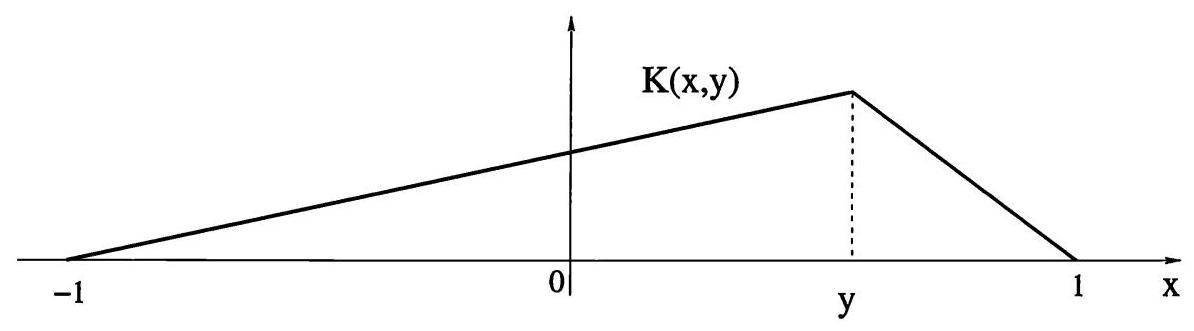
\includegraphics[width=1.0\textwidth]{images/bo_d6ik6nn7aajc739ct1l0_83_147_230_1194_331_0.jpg}
\caption{式\eqref{eq:green-kernel}中的核函数 $K$.}
\label{fig:kernel-function-K}
\end{figure}

\begin{instance}\label{ins:two-point-bvp-compact}
对任意连续函数 $f \in  \mathcal{C}\left( \left(  {-1,1}\right)  \right)$ ，令 $u = {\Lambda f}$ 为两点边值问题的解
\begin{equation}\tag{4.10}\label{eq:two-point-bvp}
{u}^{\prime \prime }\left( x\right)  + f\left( x\right)  = 0,\;u\left( {-1}\right)  = u\left( 1\right)  = 0.
\end{equation}

注意解必唯一.事实上，若 ${u}_{1},{u}_{2}$ 均为解，则函数 $w = {u}_{1} - {u}_{2}$ 满足
\[
{w}^{\prime \prime }\left( x\right)  = 0,\;w\left( {-1}\right)  = w\left( 1\right)  = 0,
\]
故 $w\left( x\right)  \equiv  0$ .直接计算表明
\[
u\left( x\right)  = {\int }_{-1}^{x}\frac{\left( {1 + y}\right) \left( {1 - x}\right) }{2}f\left( y\right) {dy} + {\int }_{x}^{1}\frac{\left( {1 - y}\right) \left( {1 + x}\right) }{2}f\left( y\right) {dy}
\]
给出了\eqref{eq:two-point-bvp}的一个解.因此解算子 $\Lambda  : f \mapsto  u = {\Lambda f}$ 是 $\mathcal{C}\left( \left(  {-1,1}\right)  \right)$ 上的线性紧算子.它可写成\eqref{eq:integral-operator-def}的形式，其中
\begin{equation}\tag{4.11}\label{eq:green-kernel}
K\left( {x,y}\right)  \doteq \begin{cases}\frac{\left( {1 - y}\right) \left( {1 + x}\right) }{2} & \text{ if } - 1 \leq  x \leq  y, \\[5pt]  \frac{\left( {1 + y}\right) \left( {1 - x}\right) }{2} & \text{ if }y \leq  x \leq  1. \end{cases}
\end{equation}

参照图\ref{fig:kernel-function-K}，对固定 $y$ ，分段仿射映射 $x \mapsto  K\left( {x,y}\right)$ 可由以下三个方程唯一确定
\[
K\left( {-1,y}\right)  = K\left( {1,y}\right)  = 0,\;{K}_{x}\left( {y+,y}\right)  - {K}_{x}\left( {y-,y}\right)  =  - 1.
\]
\end{instance}

\section{习题}

\begin{rbhw}[index=1]
在Banach空间 $X = \mathcal{C}\left( \left(  {0,1}\right)  \right)$ 上，判断下列算子是否(i)线性、(ii)有界、(iii)紧:

(1) $\left( {\Lambda f}\right) \left( x\right)  = f\left( {\sin x}\right)$ .

(2) $\left( {\Lambda f}\right) \left( x\right)  = \sin \left( {f\left( x\right) }\right)$ .

(3) $\left( {\Lambda f}\right) \left( x\right)  = {xf}\left( x\right)$ .

(4) $\left( {\Lambda f}\right) \left( x\right)  = {xf}\left( 0\right)  + {\int }_{0}^{1}f\left( s\right) {ds}$ .

(5) $\left( {\Lambda f}\right) \left( x\right)  = y\left( x\right)$ ，其中 $y\left( \cdot \right)$ 是Cauchy问题的解
\[
{y}^{\prime }\left( x\right)  + y\left( x\right)  = f\left( x\right) ,\;y\left( 0\right)  = 0.
\]
\end{rbhw}

\begin{rbhw}
证明 ${L}^{2}\left( \left(  {0,1}\right)  \right)$ 是 ${L}^{1}\left( \left(  {0,1}\right)  \right)$ 中第一纲的向量子空间.事实上，对每个 $n \geq  1$ ，集合 ${E}_{n} \doteq  \left\{  {f : \left(  {0,1}\right)   \mapsto  \mathbb{R};{\int }_{0}^{1}{\left| f\right| }^{2}{dx} \leq  n}\right\}$ 是 ${L}^{1}$ 中无内点的闭子集.
\end{rbhw}

\begin{rbhw}
设 $X$ 为一个 Banach 空间， $\Lambda  : X \mapsto  {\ell }^{\infty }$ 为一线性算子，使得对每个 $x \in  X$ ， $\Lambda \left( x\right)  = \left( {{\Lambda }_{1}\left( x\right) ,{\Lambda }_{2}\left( x\right) ,\ldots }\right)$ 均为一有界实数列.证明:算子 $\Lambda$ 有界当且仅当每个线性泛函 ${\Lambda }_{n}$ 有界.
\end{rbhw}

\begin{rbhw}
设 $1 \leq  p \leq  \infty$ .考虑定义在整个空间 ${L}^{p}$ 上的线性算子 $\Lambda  : {L}^{p}\left( \left(  {0,1}\right)  \right)  \mapsto  {L}^{p}\left( \left(  {0,1}\right)  \right)$ ，其具有如下性质:若函数列 ${f}_{n} \in  {L}^{p}$ 几乎处处点态收敛于某个 $f \in  {L}^{p}$，则序列 $\left( {\Lambda {f}_{n}}\right) \left( x\right)$ 几乎处处收敛于 $\left( {\Lambda f}\right) \left( x\right)$ (对几乎所有的 $x \in  \left(  {0,1}\right)$ ).证明: $\Lambda$ 连续.
\end{rbhw}

\begin{rbhw}
设 $X$ 为无限维 Banach 空间， $K : X \mapsto  X$ 为一紧线性算子.若 $K$ 是单射，则 $K$ 的值域不可能是闭的.
\end{rbhw}

\begin{rbhw}
设 $X,Y,Z$ 为 Banach 空间，考虑两个线性算子 ${\Lambda }_{1} : X \mapsto \; Y,{\Lambda }_{2} : Y \mapsto  Z$ .假设其中一算子连续，另一算子紧.证明:复合算子 ${\Lambda }_{2} \circ  {\Lambda }_{1} : X \mapsto  Z$ 为紧线性算子.
\end{rbhw}

\begin{rbhw}
设 $X$ 为 Banach 空间， $\Lambda  : X \mapsto  X$ 为满足 $\Lambda  = {\Lambda }^{2}$ 的紧线性算子，即对所有 $x \in  X$ ，均有 $\Lambda \left( x\right)  = \Lambda \left( {\Lambda \left( x\right) }\right)$ .证明: $\operatorname{Range}\left( \Lambda \right)$ 是有限维的.
\end{rbhw}

\begin{rbhw}
设 $X$ 为 Banach 空间， $U \subset  X$ 为一闭凸集，且满足 $\mathop{\bigcup }\limits_{{n \geq  1}}{nU} = X$ .证明: $U$ 包含原点的一个邻域.
\end{rbhw}

\begin{rbhw}
设 $X,Y$ 为无限维 Banach 空间.若 $K : X \mapsto  Y$ 为紧线性算子，则 $K\left( X\right)  \neq  Y$ ，即 $K$ 不可能是满射.

例如，考虑如下定义的映射 $K : {\ell }^{1} \mapsto  {\ell }^{1}$ :若 $\bm{x} = \; \left( {{x}_{1},{x}_{2},{x}_{3},\ldots }\right)$ 且 $\| \bm{x}{\| }_{{\ell }^{1}} \doteq  \mathop{\sum }\limits_{{n \geq  1}}\left| {x}_{n}\right|  < \infty$ ，则 $K\bm{x} = \left( {\frac{{x}_{1}}{1},\frac{{x}_{2}}{2},\frac{{x}_{3}}{3},\ldots ,\frac{{x}_{n}}{n},\ldots }\right)$ .求一点 $\bm{y} \in  {\ell }^{1} \setminus  K\left( {\ell }^{1}\right)$ .
\end{rbhw}

\begin{rbhw}
设 $f : \mathbb{R} \mapsto  \mathbb{R}$ 是一个具有闭图像的有界函数.证明 $f$ 连续.

另一方面，构造一个单射且满射、具有闭图像但不连续的函数 $g : \mathbb{R} \mapsto  \mathbb{R}$ .
\end{rbhw}

\begin{rbhw}
设 $X,Y$ 是Banach空间.证明每个连续函数 $f : X \mapsto  Y$ (未必是线性的)均具有闭图像.

构造一个具有闭图像但不连续的有界函数 $g : \mathbb{R} \mapsto  {L}^{1}\left( \mathbb{R}\right)$ .
\end{rbhw}

\begin{rbhw}
设 $1 \leq  p < \infty$ ，并考虑所有实数列 $\bm{x} = \; \left( {{x}_{1},{x}_{2},{x}_{3},\ldots }\right)$ 构成的Banach空间 ${\ell }^{p}$，其中满足 $\| \bm{x}{\| }_{p} \doteq  {\left( \mathop{\sum }\limits_{{k \geq  1}}{\left| {x}_{k}\right| }^{p}\right) }^{1/p} < \infty$ .设 $\left( {{\lambda }_{1},{\lambda }_{2},{\lambda }_{3},\ldots }\right)$ 是一有界实数列，并定义有界线性算子 $\Lambda  : {\ell }^{p} \mapsto  {\ell }^{p}$ 如下:

\[
\Lambda \left( {{x}_{1},{x}_{2},{x}_{3},\ldots }\right)  \doteq  \left( {{\lambda }_{1}{x}_{1},{\lambda }_{2}{x}_{2},{\lambda }_{3}{x}_{3},\ldots }\right) .
\]

证明: $\Lambda$ 是紧算子当且仅当 $\mathop{\lim }\limits_{{k \rightarrow  \infty }}{\lambda }_{k} = 0$ .
\end{rbhw}

\begin{rbhw}
设 $X,Y,Z$ 为Banach空间， $B : X \times  Y \mapsto  Z$ 为双线性映射\footnote{称 $B$ 是双线性的，是指:对每个给定的 $y \in  Y$ ， $x \mapsto  B\left( {x,y}\right)$ 是线性映射；且对每个固定的 $x \in  X$ ， $y \mapsto  B\left( {x,y}\right)$ 是线性映射.}.假设 $B$ 在原点处连续.证明: $B$ 是有界的；即存在常数 $C$ ，使得
\[
\| B\left( {x,y}\right) \|  \leq  C\| x\| \| y\| \;\forall\,x \in  X,y \in  Y.
\]

\end{rbhw}

\begin{rbhw}
设 $X$ 为所有一元实变量多项式构成的向量空间，其范数为
\[
\| p\|  \doteq  {\int }_{0}^{1}\left| {p\left( t\right) }\right| {\d t}
\]
考虑如下定义的双线性泛函 $B : X \times  X \mapsto  \mathbb{R}$ :
\[
B\left( {p,q}\right)  = {\int }_{0}^{1}p\left( t\right) q\left( t\right) {\d t}
\]
证明:对每个固定的 $p \in  X$ ，映射 $q \mapsto  B\left( {p,q}\right)$ 是 $X$ 上的连续线性泛函；类似地，对固定的 $q \in  X$ ，映射 $p \mapsto  B\left( {p,q}\right)$ 是连续线性泛函.然而，证明 $B$ 并非从积空间 $X \times  X$ 到 $\mathbb{R}$ 的连续映射.我们回顾: $X \times  X$ 具有范数 $\| \left( {p,q}\right) \|  \doteq  \max \left\{  {{\int }_{0}^{1}\left| {p\left( x\right) }\right| {dx},{\int }_{0}^{1}\left| {q\left( x\right) }\right| {dx}}\right\}$ .
\end{rbhw}

\begin{rbhw}
设 $S$ 是Banach空间 $X$ 中的一个闭有界子集.假设对每个 $\varepsilon  > 0$ ，均存在一个有限维子空间 ${Y}_{\varepsilon } \subseteq  X$ ，使得
\[
d\left( {S,{Y}_{\varepsilon }}\right)  \doteq  \mathop{\sup }\limits_{{x \in  S}}d\left( {x,{Y}_{\varepsilon }}\right)  \leq  \varepsilon
\]
证明:集合 $S$ 是紧集.
\end{rbhw}

\begin{rbhw}
设 $A$ 是Banach空间 $X$ 上的有界线性算子.若对每个紧算子 $K$ 均有 ${AK} = {KA}$，则证明 $A$ 是恒等算子的标量倍数，即存在某个数 $\lambda$ ，使得 $A = {\lambda I}$ .
\end{rbhw}


\begin{rbhw}
设 $X$ 是Banach空间， $\Lambda  : X \mapsto  X$ 是其上有界线性算子.假设存在 $\varepsilon  > 0$ 及一个无限维子空间 $V \subseteq  X$ ，使得对每个 $x \in  V$ 均有 $\| {\Lambda x}\|  \geq  \varepsilon \| x\|$ .证明:算子 $\Lambda$ 不可能是紧算子.
\end{rbhw}

\begin{rbhw}
设 $X$ 为 Banach 空间， ${X}^{ * }$ 为其对偶空间.考虑一列元素 ${x}_{k} \in  X$ ，满足级数 $\mathop{\sum }\limits_{{k > 1}}\left\langle  {{x}^{ * },{x}_{k}}\right\rangle$ 对每个 ${x}^{ * } \in  {X}^{ * }$ 均收敛.证明
\[
{x}^{ * } \mapsto  \varphi \left( {x}^{ * }\right)  \doteq  \mathop{\sum }\limits_{{k \geq  1}}\left\langle  {{x}^{ * },{x}_{k}}\right\rangle
\]
是 ${X}^{ * }$ 上的有界线性泛函.
\end{rbhw}

\begin{rbhw}
在 Banach 空间 $X = \mathcal{C}\left( \left(  {0,1}\right)  \right)$ 上，考虑由下式定义的线性算子 $\Lambda  : X \mapsto  X$ :
\[
\left( {\Lambda f}\right) \left( 0\right)  = f\left( 0\right) ,\;\left( {\Lambda f}\right) \left( t\right)  = \frac{1}{t}{\int }_{0}^{t}f\left( s\right) {ds}\;\text{ for }t > 0.
\]
(i) 证明 $\Lambda$ 连续.

(ii) 证明 $\Lambda$ 是单射但不是满射.

(iii) 证明 $\Lambda$ 不是紧算子.
\end{rbhw}

\begin{rbhw}
设 $\Omega  \subset  {\mathbb{R}}^{n}$ 为开集， $g : \Omega  \mapsto  \mathbb{R}$ 为有界可测函数.仿照例 2.18，对任意 $1 \leq  p \leq  \infty$，在空间 ${L}^{p}\left( \Omega \right)$ 上考虑乘法算子 $\left( {{M}_{g}f}\right) \left( x\right)  \doteq  g\left( x\right) f\left( x\right)$ .

(i) 确定使算子 ${M}_{g}$ 为单射的函数 $g$ .

(ii) 确定使算子 ${M}_{g}$ 具有闭值域的函数 $g$ .

(iii) 确定使算子 ${M}_{g}$ 为紧算子的函数 $g$ .
\end{rbhw}

\begin{rbhw}
构造一个例子，说明:对无穷维 Banach 空间 $X$ ，所有单射的有界线性算子 $\Lambda  : X \mapsto  X$ 的集合未必是全体有界线性算子空间 $\mathcal{B}\left( {X;X}\right)$ 中的开集.

类似地，说明值域稠密的有界线性算子集合在 $\mathcal{B}\left( {X;X}\right)$ 中也未必是开集.
\end{rbhw}

\begin{rbhw}
设 $X,Y$ 为 Banach 空间， $\Lambda  : X \mapsto  Y$ 为连续线性双射.

(i) 证明存在 $\beta  > 0$ ，使得
\[
\| {\Lambda x}\|  \geq  \beta \| x\| \forall\,x \in  X.
\]

(ii) 设 $\Psi  \in  \mathcal{B}\left( {X;Y}\right)$ 为任一范数为 $\| \Psi \|  < \beta$ 的有界线性算子.利用压缩映射原理，证明:对任意 $f \in  Y$ ，方程
\[
u = {\Lambda }^{-1}\left( {f - {\Psi u}}\right)
\]
有唯一解.

(iii) 证明:在Banach空间 $\mathcal{B}\left( {X;Y}\right)$ 中，所有双射算子构成的集合是开集.
\end{rbhw}

\begin{rbhw}
回顾第2章例2.6与2.7中引入的空间，定义算子 $\Lambda  : {\ell }^{\infty } \mapsto  {\ell }^{\infty }$ 如下: ${\Lambda x} = y = \left( {{y}_{1},{y}_{2},{y}_{3},\ldots }\right)$ ，其中
\begin{equation}\tag{4.12}\label{eq:cesaro-mean}
{y}_{n} \doteq  \frac{1}{n}\mathop{\sum }\limits_{{i = 1}}^{n}{x}_{i}
\end{equation}

(i) 证明 $\Lambda$ 是有界线性算子，并计算其范数. $\Lambda$ 是紧算子吗？

(ii) 考虑如式\eqref{eq:cesaro-mean}所定义的算子 $\Lambda$ ，但作用于绝对可和序列空间 ${\ell }^{1}$ 上. $\Lambda$ 是有界线性算子吗？它是否紧？
\end{rbhw}

\begin{rbhw}
设 $X,Y$ 为向量空间，且 $Y \subseteq  X$ .假设存在范数，使得 $\left( {X\;;\;\|  \cdot  {\| }_{X}}\right)$ 与 $\left( {Y\;;\;\|  \cdot  {\| }_{Y}}\right)$ 均为Banach空间，且满足
\[
\| y{\| }_{X} \leq  C \cdot  \| y{\| }_{Y}\;\forall\,y \in  Y.
\]

(i) 若 $Y = X$ ，证明两种范数 $\|  \cdot  {\| }_{X}$ 与 $\|  \cdot  {\| }_{Y}$ 等价，即存在常数 ${C}^{\prime }$ ，使得 $\| x{\| }_{Y} \leq  {C}^{\prime } \cdot  \| x{\| }_{X}$ .

(ii) 若 $Y \neq  X$ ，证明 $Y$ 是 $X$ 中的第一纲集.即每个集合 ${S}_{n} \doteq  \left\{  {y \in  Y;\| y{\| }_{Y} \leq  n}\right\}$ 均为 $X$ 的闭集且无处稠密.
\end{rbhw}
